\begin{figure}
  \centering
  \vspace*{-0.5cm}
  \hspace*{1cm}
  \begin{tikzpicture}
    \node at (0, 0){
      \includegraphics[width=6cm]{experiments/3d/vae_occ/easy_15/random}
    };
    
    \draw[-,dashed] (3.25, -2.5) -- (3.25,3);
    
    \node at (6.5, 0){
      \includegraphics[width=6cm]{experiments/3d/vae_occ/easy_30/random}
    };
    
    \node at (10,0) {
      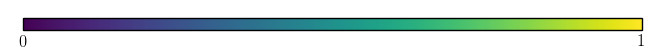
\includegraphics[height=5cm]{experiments/3d/vae_occ/easy_15/colorbar}
    };
    
    \node at (0, 3) {\begin{tabular}{c}$Q = 15$\\random samples\end{tabular}};
    \node at (6.5, 3) {\begin{tabular}{c}$Q = 30$\\random samples\end{tabular}};
  \end{tikzpicture}
  \vskip -4px

  % TODO short caption
  \caption{Random samples for \VAEs trained on the 3D cuboids dataset
  using $Q = 15$ and $Q = 30$. Although random samples are to be judged with
  caution, we find the model with $Q = 15$ generates more reasonable random
  samples. Again, we show horizontal slices of the volumes, in particular
  heights $8 + 2i$ for $0 \leq i < 8$.}
  \label{fig:appendix-experiments-3d-vae-qual-1}
\end{figure}
% \begin{figure}
%   \centering
%   \begin{tikzpicture}
%     \node at (0, 1.2){
%       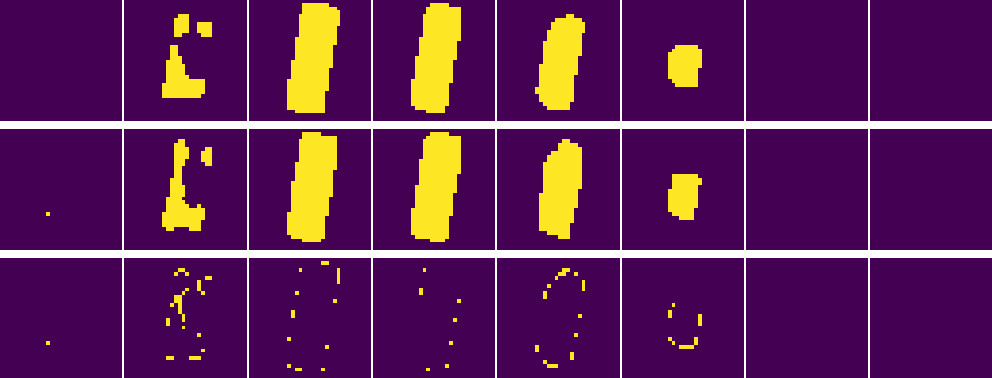
\includegraphics[width=6cm]{experiments/3d/vae_occ/easy_15/results_2}
%     };
%     \node at (0, -1.2){
%       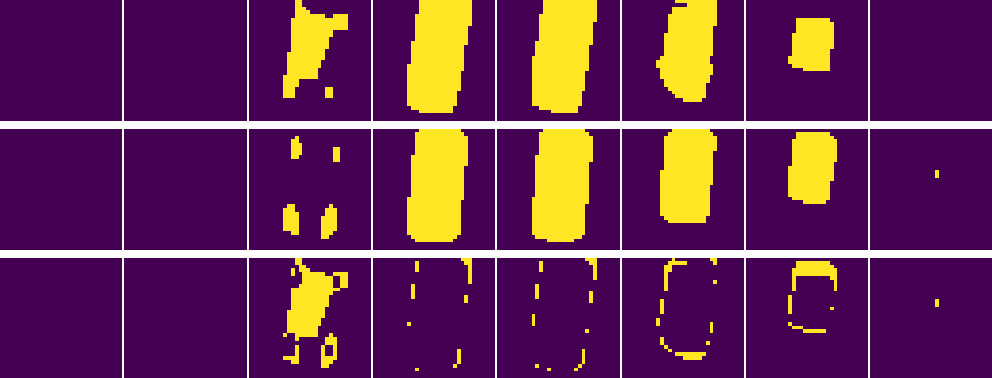
\includegraphics[width=6cm]{experiments/3d/vae_occ/easy_15/results_3}
%     };
    
%     \draw[-,dashed] (3.25, -8) -- (3.25,3);
    
%     \node at (6.5, 1.2){
%       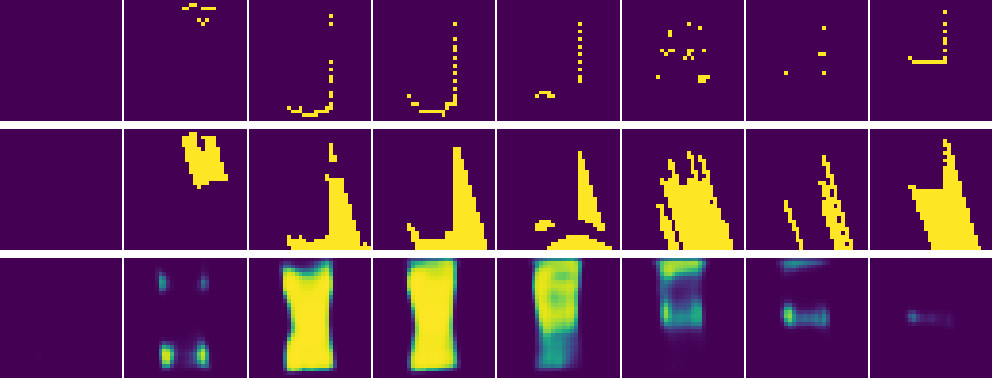
\includegraphics[width=6cm]{experiments/3d/vae_occ/easy_15/results_4}
%     };
    
%     \node at (0, 3) {\begin{tabular}{c}reconstruction\\occupancy\end{tabular}};
%     \node at (6.5, 3) {\begin{tabular}{c}reconstruction\\occupancy\end{tabular}};
    
%     \draw[-,dashed] (-3.5, -2.5) -- (10, -2.5);
    
%     \node at (-3.5,-5.1) {
%       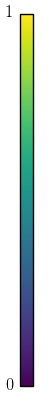
\includegraphics[height=5cm]{experiments/3d/vae_occ_sdf/colorbar_0}
%     };
    
%     \node at (0, -3.9){
%       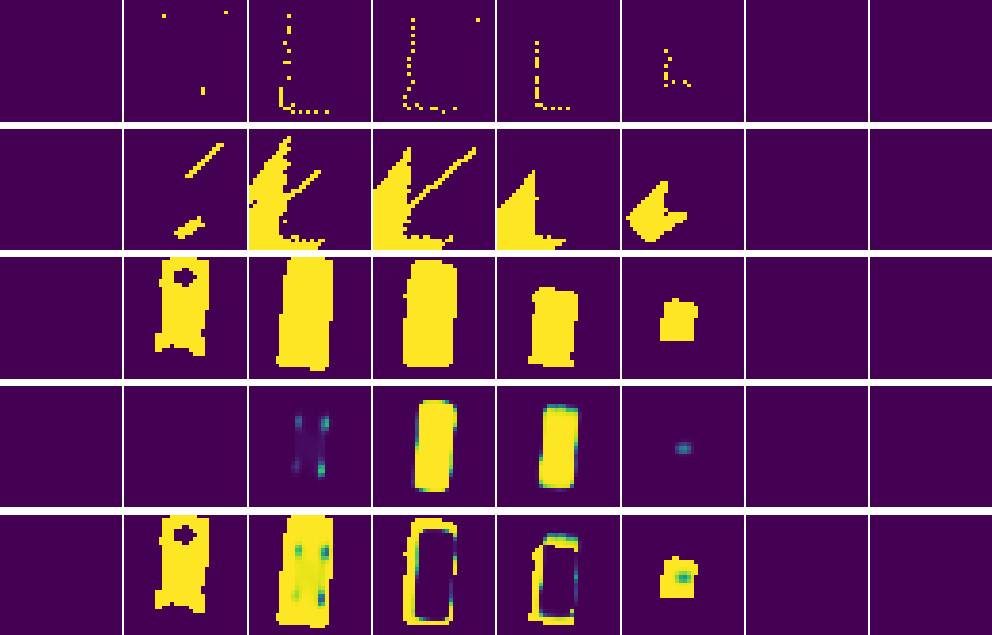
\includegraphics[width=6cm]{experiments/3d/vae_occ_sdf/easy_15/results_0_0}
%     };
%     \node at (0, -6.3){
%       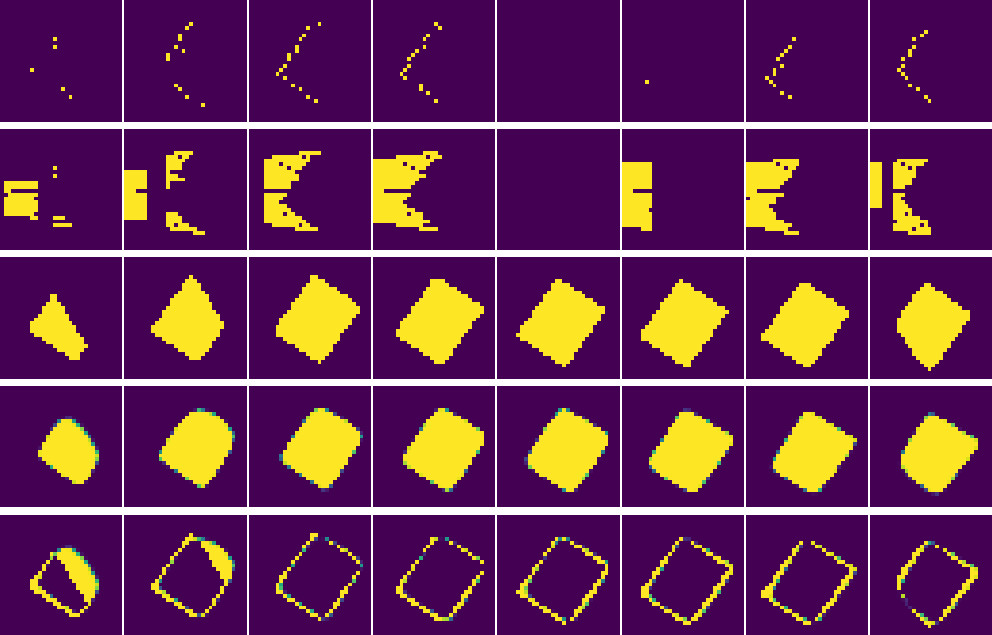
\includegraphics[width=6cm]{experiments/3d/vae_occ_sdf/easy_15/results_1_0}
%     };
    
%     %\draw[-,dashed] (3.25, -3) -- (3.25,3);
    
%     \node at (6.5, -3.9){
%       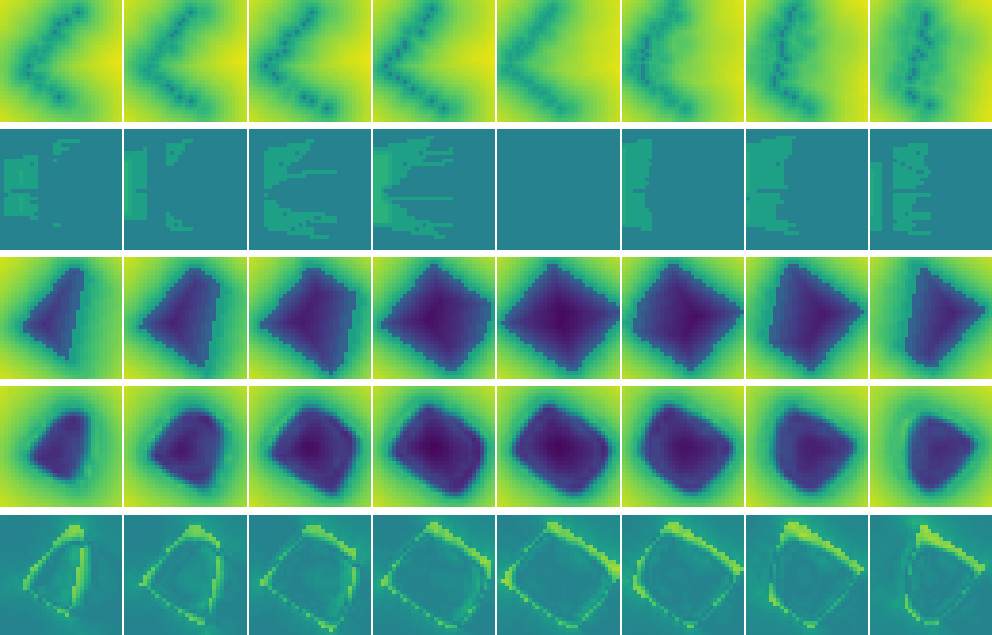
\includegraphics[width=6cm]{experiments/3d/vae_occ_sdf/easy_15/results_0_1}
%     };
%     \node at (6.5, -6.3){
%       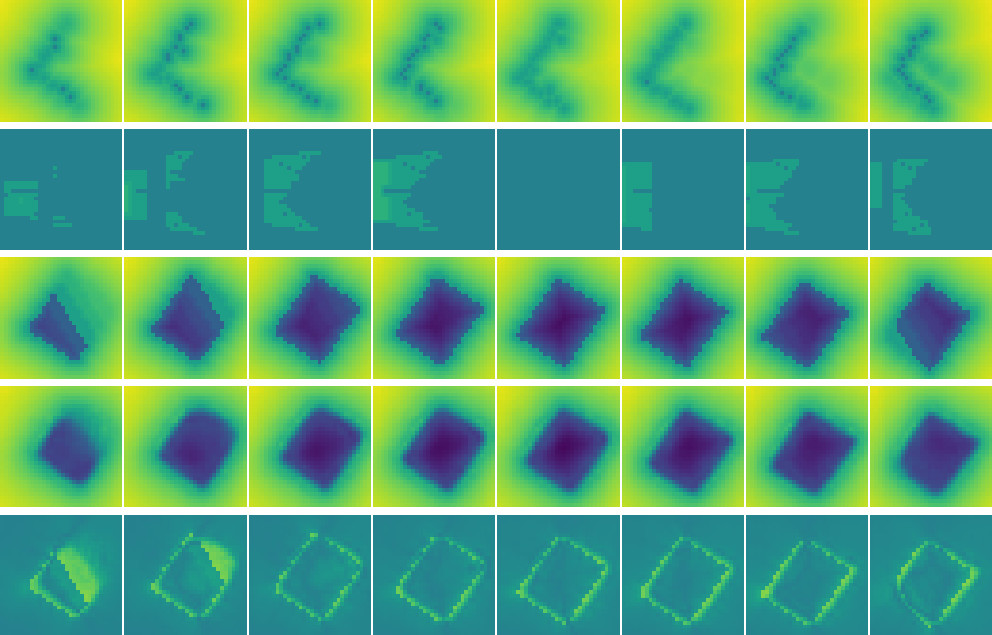
\includegraphics[width=6cm]{experiments/3d/vae_occ_sdf/easy_15/results_1_1}
%     };
    
%     \node at (10,-5.1) {
%       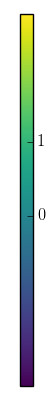
\includegraphics[height=5cm]{experiments/3d/vae_occ_sdf/colorbar_1}
%     };
   
%     \node at (0, -8) {\begin{tabular}{c}reconstruction\\occupancy\end{tabular}};
%     \node at (6.5, -8) {\begin{tabular}{c}reconstruction\\signed distance functions\end{tabular}};
%   \end{tikzpicture}
  
%   % TODO short caption
%   \caption{Illustration of the learned reconstruction capabilities for $Q = 15$
%   and a \VAE trained on occupancy only (top) and one trained on both occupancy
%   and signed distance functions bottom. Both models exhibit low reconstruction error,
%   but we find that the model trained on both modalities is slightly more uncertain
%   in its predictions; this can especially be seen in the occupancy case.
%   Following Figure \ref{fig:appendix-experiments-3d-vae-qual-1} we show height slices
%   of the corresponding volumes.}
%   \label{fig:appendix-experiments-3d-vae-qual-2}
% \end{figure}
